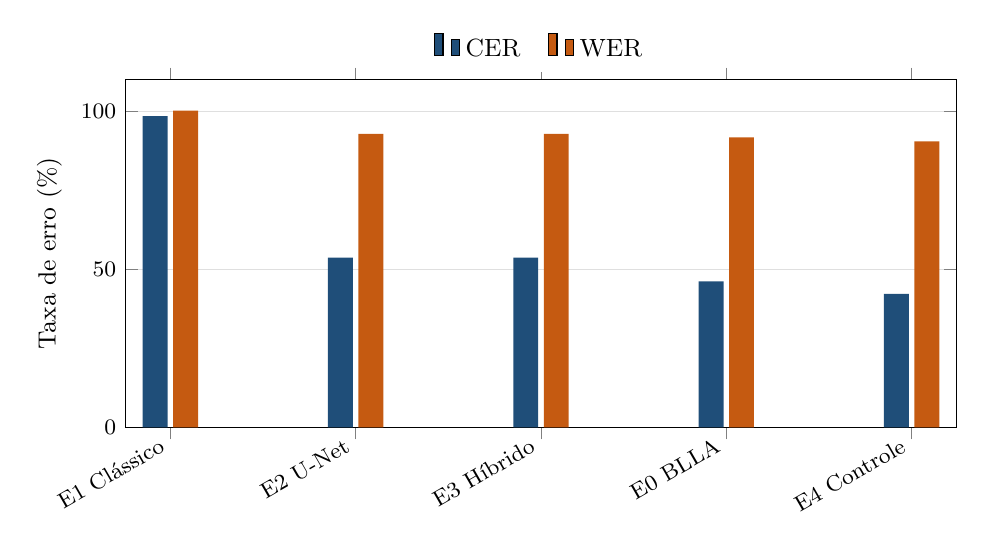
\begin{tikzpicture}
\begin{axis}[
  ybar,
  bar width=9pt,
  width=\linewidth,
  height=6cm,
  xtick={0,...,4},
  xticklabels={{E1 Clássico},{E2 U-Net},{E3 Híbrido},{E0 BLLA},{E4 Controle}},
  ylabel={Taxa de erro (\%)},
  /pgf/number format/use comma,
  /pgf/number format/precision=1,
  /pgf/number format/fixed,
  ymajorgrids,
  grid style={gray!25},
  enlarge x limits=0.06,
  tick label style={font=\footnotesize},
  label style={font=\small},
  x tick label style={rotate=30, anchor=east},
  ymin=0,
  ymax=110,
  legend style={at={(0.5,1.02)}, anchor=south, legend columns=-1, draw=none, font=\small, /tikz/every even column/.append style={column sep=8pt}}
]
\addplot[fill={rgb,255:red,31;green,78;blue,121}, draw=none] coordinates {(0,98.4543) (1,53.7097) (2,53.7097) (3,46.1601) (4,42.2063)};
\addplot[fill={rgb,255:red,197;green,90;blue,17}, draw=none] coordinates {(0,100.1546) (1,92.8130) (2,92.8130) (3,91.7311) (4,90.4173)};
\legend{CER,WER}
\end{axis}
\end{tikzpicture}
